\title{Open Sound Controll}
\author{
        Michael Lazarski \\
                Studiengang Media Systems\\
}
\date{\today}
\documentclass[a4paper, 12pt]{article}
\usepackage[ngerman]{babel}
\usepackage[utf8]{inputenc}
\usepackage{graphicx}
\usepackage{float}
\usepackage{url}
\usepackage{hyperref}
\usepackage{textcomp}
\pagestyle{headings}

\begin{document}
\maketitle

\newpage
\tableofcontents
\newpage


\section{Geschichte}
\subsection{Musical Instrument Digital Interface}
Die Geschichte von Open Sound Control beginnt mit MIDI (Musical Instrument Digital Interface).
Also am Anfang der 1980er Große Synthesiyer Manufakturen beginnen MIDI als Standart Protokoll zu Implementieren in ihre Hardware wurde dies damals als eine Revolution in der Musik Industrie angesehen. Nur mit einem Computer, einem Midi Controller und der dazugehöirgen Software konnte ein Musiker aufnehmen, Komponieren und mischen ohne zusätzliches Werkezug. Midi wird bis heute noch in der Musikindustrie benutzt. 
\paragraph{Wie Midi Funktioniert}

MIDI ist eine unidirektionale Schnittstelle zur seriellen Datenübertragung. Midi hat keine Datenflusskontrolle. Die Übertragungsgeschwindigkeit beträgt 31250 Bit/s. \cite{MIDI} \\
\\
Es gibt 3 verschiedene Midi Anschlüsse 
\begin{itemize}
  \item MIDI-IN: Hiermit empfängt der MIDI Controller Signale
  \item MIDI-OUT: Hiermit sendet der MIDI-Controller Signale
  \item MIDI-THRU: Sendet die ankommenden Signale vom MIDI-IN port einfach weiter ohne sie weiter zu verarbeiten
\end{itemize}
 \begin{figure}[htbp]
  \centering
  \fbox{
    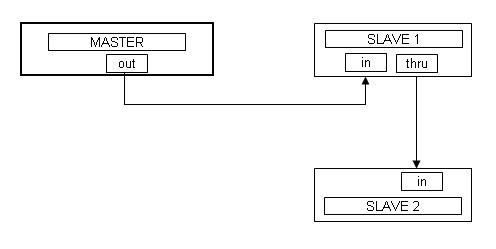
\includegraphics{mms.jpg}
  }
  \caption[MIDI Master Slave \cite{MMS}]{MIDI Master Slave} 
  \label{fig:mms}
\end{figure}
Midi funktioniert nach einem Master-Slave-Prinzip ~\ref{fig:mms}.
Will man mit einem Midi-Keyboard(Master) einen Synthesizer(Slave) steuern, so verbindet man die MIDI-OUT Buchse des Masters mit der MIDI-IN Buchse des Slaves. Möchte man nun noch einen zweiten Slave hinzufügen so schließt man ein Kabel zwischen dem MIDI-THRU des ersten Slaves mit der MIDI-IN Buchse des zweiten Slaves.

\subsubsection{Nachteile von MIDI}
MIDI hat ein paar sehr frustrierende Nachteile:
\begin{itemize}
  \item Serieller transport der Daten. Die Daten müssen erst Sequentiel geordnet werden.
  \item Langsame übertragungs raten. Sehr Problemantisch bei großen Datenmengen.
  \item Pitch wird in Integern dargestellt.
  \item Tendiert zu Keyboard Conrtolleren da Wind, Gittaren und andere Instrumente schwer zu Implementieren sind.
  \item Integer representation von Controller values. Dies kann zu ungenauigkeit führen beim einstellen von feinen paramtern.
  \item Ungenau Zeitauflösung. Diese wird auch wieder in Integern angegeben.
  \item MIDI benötig Spezielle Hardware. 
\end{itemize}
\subsection {Zeta Instrument Processor Interface}
1994 wurde von der Firma Zeta Instruments und einer Research Gruppe der University of California das Zeta Instrument Processor Interface (kurz ZIPI) vorgestellt. Es sollte MIDI ablössen und war aufdem OSI-Model aufgebaut. ZIPI konnte sich nie wirklich durchsetzen. MIDI hat eine Peer-to-Peer Architektur. ZIPI baute auf eine Stern Architektur mit einem HUB in der Mitte als zentrale Anlaufsstelle. Das hatte den vorteil das man einfach Geräte aus dem HUB entfernen konnte. ZIPI ist auch unabhängig von einer Physikalischen Implementierung. Das alles hat aber nicht geholfen da das Adressierungschema zu komplex war. Es mussten 1016127 Synth zustände geregelt werden im ZIPI Controller. Zum vergleich hatte midi nur 16 Kanäle die zwischen 12 und 128 zuständen hatten.
Es gibt bis heute keine Kommerziel vertriebenen Geräte die ZIPI unterstützen.
\newpage
\subsection{Open Sound Control}

\section{Results}\label{results}
In this section we describe the results.

\section{Conclusions}\label{conclusions}
We worked hard, and achieved very little.
\newpage
\renewcommand{\refname}{REFERENCES}
\bibliographystyle{plainnat}
\bibliography{evt}

\listoffigures
\end{document}
This is never printed
